
\documentclass[twocolumn, a4paper]{ieicejsp}
\usepackage{newenum}
\usepackage{comment}
\usepackage{ascmac}
\usepackage{amsmath}
\usepackage{amssymb}
\usepackage{amsfonts}
\usepackage[dvipdfmx]{graphicx}
\usepackage{multirow}
\usepackage{here}
\usepackage{bm}
\usepackage{epsfig}
\usepackage{array}
\usepackage{caption}
\usepackage{url}

\newcommand{\fmusic}{f_{\mathrm{MUSIC}}}
\newcommand{\fprev}{f_{\mathrm{prev}}}
\newcommand{\fcurr}{f_{\mathrm{curr}}}

\title{PPG信号を用いた動脈血圧波形予測のための \\ 
ドメイン敵対的学習による深層生成モデル
  {\normalsize \\ Deep generative model with domain adversarial training for predicting \\ arterial blood pressure waveform from photoplethysmogram signal}}
  \author{
    権藤陸 \\ Riku Gondo
  }
 \affliate{
    慶應義塾大学 理工学部$^1$ \\
    Faculty of Science and Technology, Keio university
}

\begin{document}
\maketitle

{\small
\section{はじめに}
長期的な血圧モニタリングは,個人の健康状態の変化を動的に反映することができ,潜在的な疾患の警告と予防に大きな意味を持つ\cite{intro1} \cite{intro2}.しかし,現在の血圧測定の主流は上腕を圧迫するカフをベースとした方法であり,不便であるため利用シーンが限られる.一方で近年,ウェアラブルセンサを用いた連続的な血圧モニタリングはが注目を集めており,特にPPG(Photoplethysmogram)センサは,その安価さと手首や指先で信号を測定できる利便性から,血圧測定など幅広い応用が期待されている\cite{intro3} \cite{intro4}.PPG信号から動脈血圧波形を生成できれば,血管に対し侵襲的に血圧を計測する方法の代替として,感染の危険性がなく,より安全であることから,このアプローチは潜在的な応用価値を持つ\cite{intro5}.

一方で,PPG信号と血圧の波形は被験者の健康状態によって大きく左右されてしまい,特に集中治療室患者で深刻である.このような個人差は,血圧予測を困難にさせる.

これらの事実を踏まえ,我々は,動脈血圧波形予測のための,データの個人差を考慮した深層生成モデルを開発した.

\vspace{-0.2cm}
\section{従来法}
\subsection{特徴量を手動で設定する機械学習による血圧予測}
Xingらは,FFTに基づくPPG信号の振幅と位相情報を用いて,多層パーセプトロンによって,1拍ごとの血圧を予測している\cite{ML}.

この研究では,特徴量の抽出を波形の特徴点の位置に依存しており,高品質のデータが必要である.そのため,複雑な特徴抽出や選択・変換処理に加え,データの品質を確保するための精緻な前処理やスクリーニングが必要になる点が課題である.

\vspace{-0.4cm}
\subsection{特徴量を自動で学習する深層学習による血圧予測}
Eomらは,VGGNetという畳み込みモデルとBi-GRU層を重ねたモデルを提案した.このモデルでは,時間方向に沿った特徴ベクトルの重要度を定量化するためにセルフアテンション機構が利用されている\cite{DL}.

このような深層学習ベースのアプローチは,各タスク(SBP\footnote{SBP: Systolic Blood Pressure},DBP\footnote{DBP: Diastolic Blood Pressure},またはMBP\footnote{MBP: Mean Blood Pressure})予測に対して独立した予測モデルを学習する従来の機械学習ベースのアプローチとは異なり,1つのモデルのみで事足りる.しかし,SBP, DBP, MBPの間で損失スケールが異なると,モデルの学習に支障をきたすという別の問題が生じる.

\vspace{-0.4cm}
\subsection{ABP波形予測}
前提として,我々の知る限り,血圧波形を直接予測した研究はほとんどない.Ibetehaz\cite{ABP1}らは,医用画像分野の古典的なネットワークであるUNet\cite{ABP2}をディープスーパービジョンの概念と組み合わせて,PPG信号からABP波形の生成に適用している.しかし,上記の研究のいずれも異なる被験者から得られたデータ間の個人差を考慮していない.

\vspace{-0.2cm}
\section{提案法}

\subsection{RDAE(Regularized Deep Autoencoder)}
RDAEは教師ありディープオートエンコーダであり,損失関数に正則化項を加えることで,ドメイン敵対的学習を実現したモデルである.入出力データである生理信号の周期性とパターン反復性を考慮し,RNN(Recurret Neural Network)と比較して計算量が小さい1次元畳み込み層を採用した.

本稿では,各個人の記録をドメインとみなす.そして,RDAEでは,エンコーダと分類器が敵対的に学習を進めることを"ドメイン敵対的学習"と呼んでいる.具体的には,エンコーダは信号変換誤差を最小化し,分類器の識別能力を弱らせる方向に学習を進め,分類器は,各PPG信号の潜在表現の所属クラス(個人)を識別する方向に学習を進める.

本モデルが最適化すべき目的関数は以下のようになる.
\vspace{-0.2cm}
\begin{equation}
  l(\phi, \varphi, \pi) = \mathrm{E}_{(x, y) \sim P_{data}} L_r(D_{\varphi} (E_{\phi}(x)), y) - \lambda \cdot L_d (D_\pi (E_{\phi} (x)), d_x)
\end{equation}
第一項は信号変換損失を表し,$L_r$はMAE(Mean Absolute Error)を表し,$P_{data}$は
$x, y$は未知の$X \mathrm{x} Y$の事前分布である$P_{data}$から取り出されたサンプルである.第二項はドメイン分類器に対する分類損失を表し,$L_d$は交差エントロピー誤差で計算される.$\lambda$はハイパーパラメータで,二項の重みを決定する.

そして,各パラメータの更新式は以下のように表される.
\vspace{-0.2cm}
\begin{eqnarray}
  \pi & \leftarrow & \pi - \alpha \lambda \cdot \nabla_{\pi} L_d, \\
  \varphi & \leftarrow & \varphi - \alpha \cdot \nabla_{\varphi} L_r, \\
  \phi & \leftarrow & \phi - \alpha \cdot \nabla_{\phi} (L_r - \lambda \cdot L_d)
\end{eqnarray}

\begin{enumerate}
\item エンコーダのパラメータ$\phi$,デコーダのパラメータ$\varphi$,ドメイン分類器のパラメータ$\pi$を全て初期化する.
\item バッチサイズ分のサンプルを取り出し,潜在ベクトル$z$を計算する.
\item ドメイン分類器の出力を計算する.
\item 分類器の出力に対する勾配を計算し,分類器のパラメータ$\pi$を(2)式に従い更新する.
\item 2をもう一度実行し,分類器とデコーダの出力を計算する.
\item 分類器とデコーダの出力に対する勾配を計算し,エンコーダのパラメータ$\phi$を(3)式に従い更新する.
\item デコーダの出力に対する勾配を計算し,デコーダのパラメータ$\varphi$を(4)式に従い更新する.
\item 1-7を推定精度が収束するか,最大エポック数を超えるまで繰り返す.

\end{enumerate}

\vspace{-0.4cm}
\subsection{キャリブレーション}
キャリブレーションはソースドメインでの学習モデルをターゲットドメインに適合させる手法である.
確立されたヘルスケア規格は,評価プロセス中のテストデバイスのキャリブレーションを許可していないが,実際のアプリケーションでは,個人の血圧関連データが継続的に測定・記録されるため,個人の履歴データを用いてモデルをキャリブレーションすることは容易であると考えられる.
本研究では,各テストレコードについてその最初の8サンプルを用いて,学習済みのモデルをさらに学習(キャリブレーション)する.

\vspace{-0.2cm}
\section{実験}
1227人の被験者からPPG信号を検出し,ABP波形を推定した.MIMIC$\mathrm{I}\hspace{-1.2pt}\mathrm{I}$データセット\cite{dataset}に含まれるPPG信号とABP信号を真値として以下に示すように精度指標を計算した.

\begin{itemize}
  \item 平均絶対誤差(MAE: Mean Absolute Error)
  \begin{equation}
    MAE = \frac{1}{N} \sum_{i=1}^{N} |p_i - \hat{p_i}|
  \end{equation}
  \item 平均誤差(ME: Mean Error)
  \begin{equation}
    ME = \frac{1}{N} \sum_{i=1}^{N} |p_i - \hat{p_i}|
  \end{equation}
  \item 標準偏差(STD: Standard Deviation)
  \begin{equation}
    STD = \sqrt{\frac{\sum_{i=1}^{N} (\hat{p_i} - \overline{p_i})^2}{N}}
  \end{equation}
\end{itemize}
ただし,
\begin{itemize}
  \item $N$: 被験者数
  \item $p_i$: 血圧の真値
  \item $\hat{p_i}$: 血圧の推定値
  \item $\overline{p_i}$: 血圧推定値の平均値
\end{itemize}

図1は,推定したABP波形と真値の比較である.赤で示された推定波形が青の真値の波形を高精度に予測できていると確認できる.

\begin{figure}[H]
  \begin{center}
    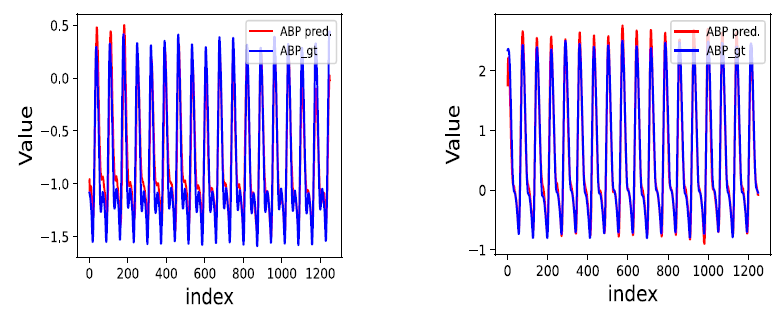
\includegraphics[width=7cm]{./result_abpwave.png}
    \caption{\small 推定ABP波形と真値の比較}
  \end{center}
\end{figure}

表1は,通常のディープオートエンコーダ(DAE)とドメイン敵対的学習が含まれたRDAE,そしてキャリブレーションありのRDAEの比較である.結果は平均値で示され,括弧内は標準誤差である.表の下へ行くほど,3つの指標(MAE, ME, STD)の標準誤差が小さくなるため,ドメイン敵対的学習によるロバスト性向上が確認できる.同様に,MAEが小さくなることで,キャリブレーションによるモデルの予測精度向上が確認できる.

\begin{figure}[H]
  \begin{center}
    \caption*{{\small 表1 ドメイン敵対的学習とキャリブレーションの精度比較}}
    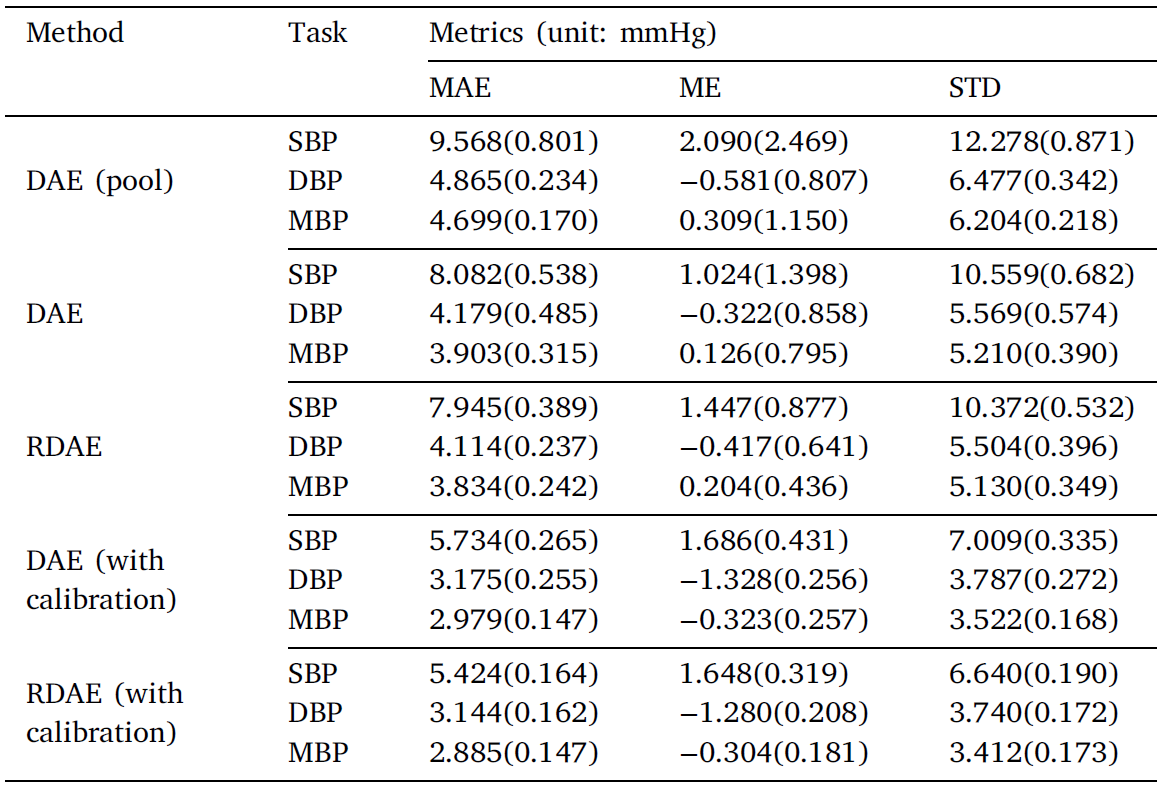
\includegraphics[width=7cm]{./result_ablation.png}
  \end{center}
\end{figure}

表2は,提案法と従来法のMAEとパラメータ数を比較したものである.表から,提案法は従来法に予測精度が少し劣る部分もあるが,パラメータ数の小さいモデルとなっていることが確認できる.

\begin{figure}[H]
  \begin{center}
    \caption*{\small 表2 提案法と従来法の比較}
    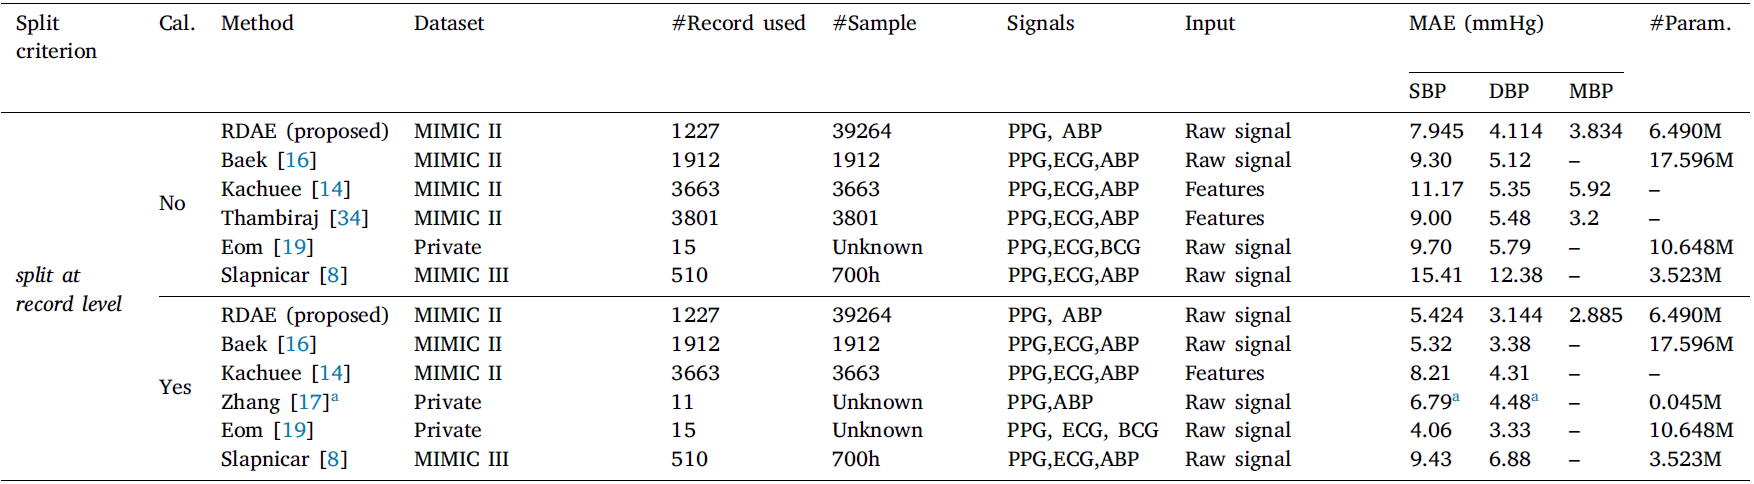
\includegraphics[width=9cm]{./result_other_systems.png}
  \end{center}
\end{figure}


\vspace{-0.2cm}
\section{おわりに}
本稿では,PPG信号のみを用いて,ドメイン敵対的学習とキャリブレーションを用いて,データの個人差を考慮した高精度なRDAEを提案した.ドメイン敵対的学習とキャリブレーションにより,予測精度とロバスト性が改善され,従来法と比較してパラメータ数の少ないモデルを開発できたことを確認した.



\vspace{-0.1cm}
%{\scriptsize
{\scriptsize
\begin{thebibliography}{9}

\bibitem{intro1} G. Thambiraj, U. Gandhi, V. Devanand, M. Umapathy, Noninvasive cuffless
blood pressure estimation using pulse transit time, Womersley number, and
photoplethysmogram intensity ratio, Physiol. Meas. 40 (2019)

\bibitem{intro2} I. Sharifi, S. Goudarzi, M.B. Khodabakhshi, A novel dynamical approach in
continuous cuffless blood pressure estimation based on ECG and PPG signals,
Artif. Intell. Med. 97 (2018)

\bibitem{intro3} Q. Zhu, X. Tian, C.W. Wong, M. Wu, ECG reconstruction via PPG: A pilot
study, in: 2019 IEEE EMBS International Conference on Biomedical and Health
Informatics, BHI, IEEE, 2019, pp. 1–4

\bibitem{intro4} J. Allen, Photoplethysmography and its application in clinical physiological
measurement, Physiol. Meas. 28 (2007) R1–39

\bibitem{intro5} G. Martínez, N. Howard, D. Abbott, K. Lim, R. Ward, M. Elgendi, Can photoplethysmography
replace arterial blood pressure in the assessment of blood
pressure? J. Clin. Med. 7 (2018) 316

\bibitem{ML} X.M. Xing, M.S. Sun, Optical blood pressure estimation with photoplethysmography
and FFT-based neural networks, Biomed. Opt. Express 7 (2016) 3007–3020

\bibitem{DL} H. Eom, D. Lee, S. Han, Y. Hariyani, Y. Lim, I. Sohn, K. Park, C. Park,
End-to-End deep learning architecture for continuous blood pressure estimation
using attention mechanism, Sensors 20 (2020) 2338

\bibitem{ABP1} N. Ibtehaz, M.S. Rahman, PPG2ABP: Translating photoplethysmogram (PPG)
signals to arterial blood pressure (ABP) waveforms using fully convolutional
neural networks, 2020, arXiv:arXiv:2005.01669.

\bibitem{ABP2} O. Ronneberger, P. Fischer, T. Brox, U-Net: Convolutional networks for
biomedical image segmentation, in: International Conference on Medical Image
Computing and Computer-Assisted Intervention, Vol. 9351, Springer, 2015, pp.
234–241 using a spectro-temporal deep neural network, Sensors 19 (2019)
3420
\bibitem{dataset} \url{https://archive.ics.uci.edu/ml/datasets/Cuff-Less+Blood+Pressure+Estimation}
\end{thebibliography}
}

\end{document}
